% !TEX root = Master.tex


By viewing the sales trends separately for each key category cluster, we can observe in \autoref{fig:ts_log_sales_kcc} that, among the weekly noise, they climax similarly. Just like in the previous section, those peaks come about primarily during the big promotions weeks. To put it into perspective, we can see logarithmic sales behaviour in \autoref{fig:boxplot_log_sales_kcc}, were patterns are quite similar although they differ strongly in volume. \\

 \begin{figure}[H]
\centering
\begin{subfigure}{.45\textwidth}
  \centering
  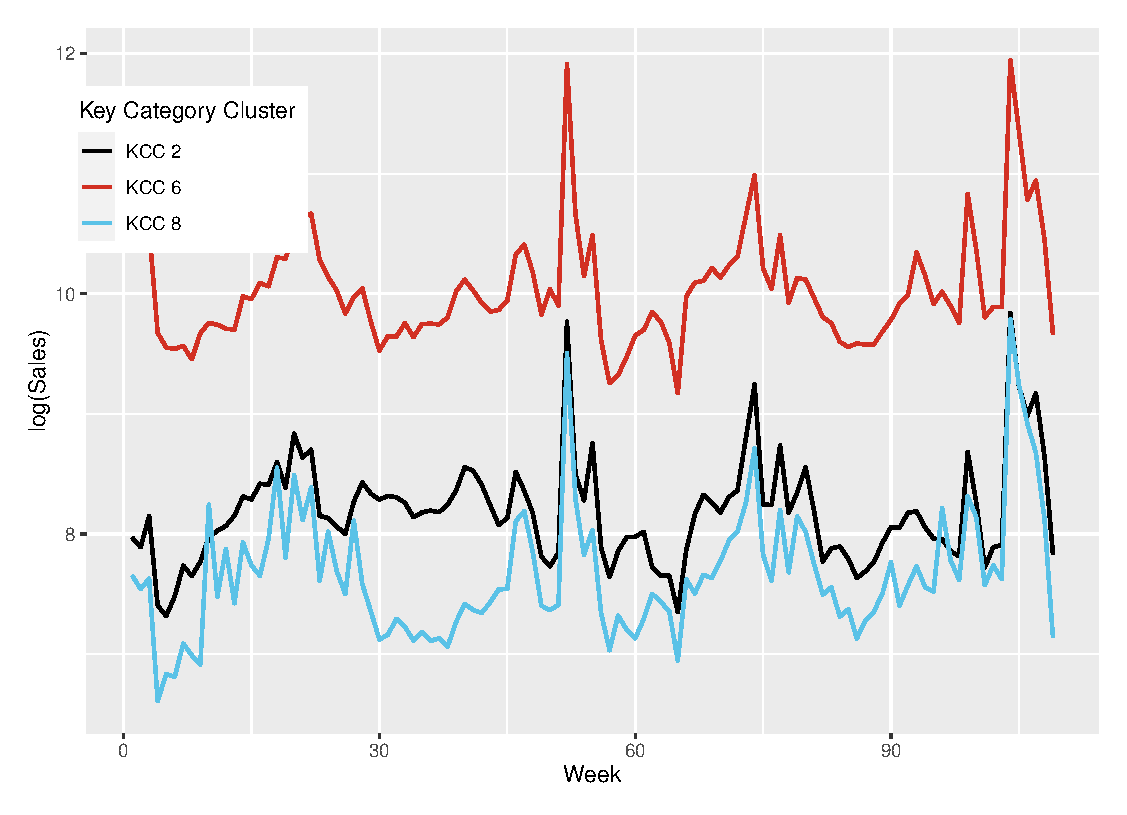
\includegraphics[width=\linewidth]{figures/ts_log_sales_kcc.eps}
  \caption{Time series of log(Sales) per KCC}
  \label{fig:ts_log_sales_kcc}
\end{subfigure}
\begin{subfigure}{.45\textwidth}
  \centering
  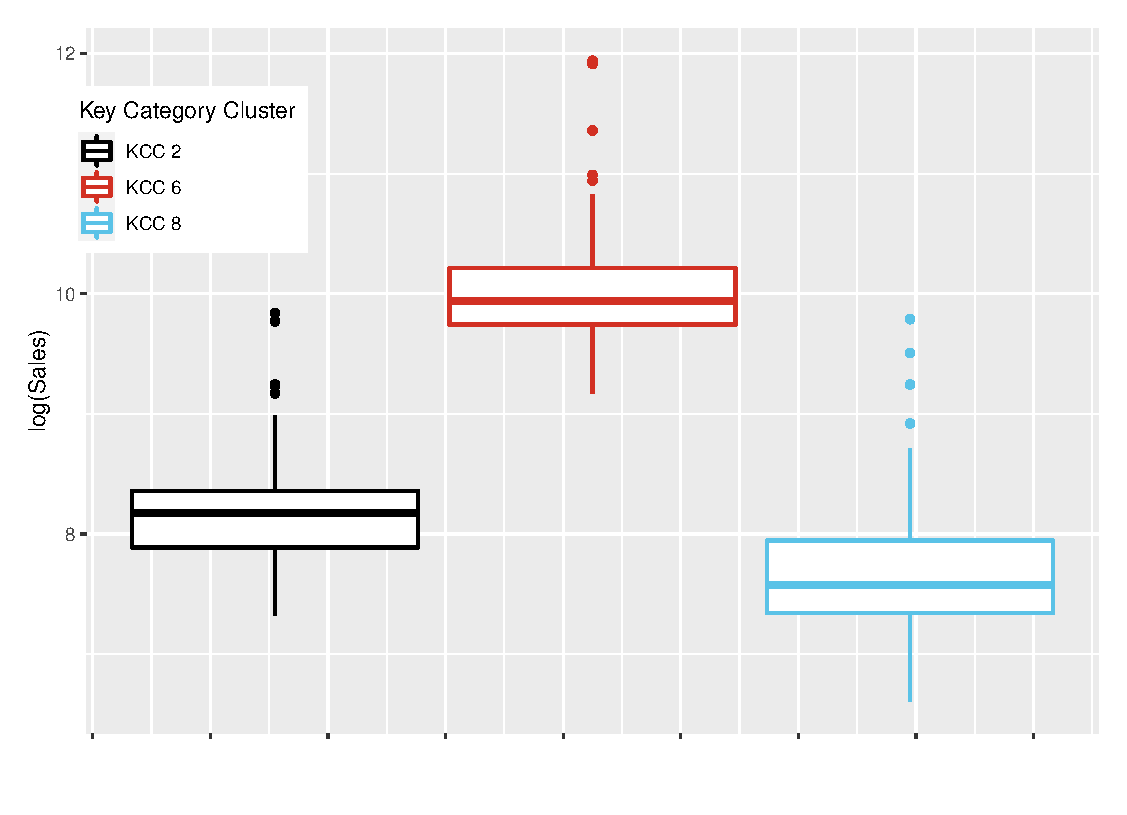
\includegraphics[width=\linewidth]{figures/boxplot_log_sales_kcc.eps}
  \caption{Boxplots of log(Sales) per KCC}
  \label{fig:boxplot_log_sales_kcc}
\end{subfigure}
\caption{Time series and boxplot showing logarithmized sales of the key category clusters}
\label{fig:kcc_ts_and_boxplot}
\end{figure} 




\begin{figure}[H]
\centering
  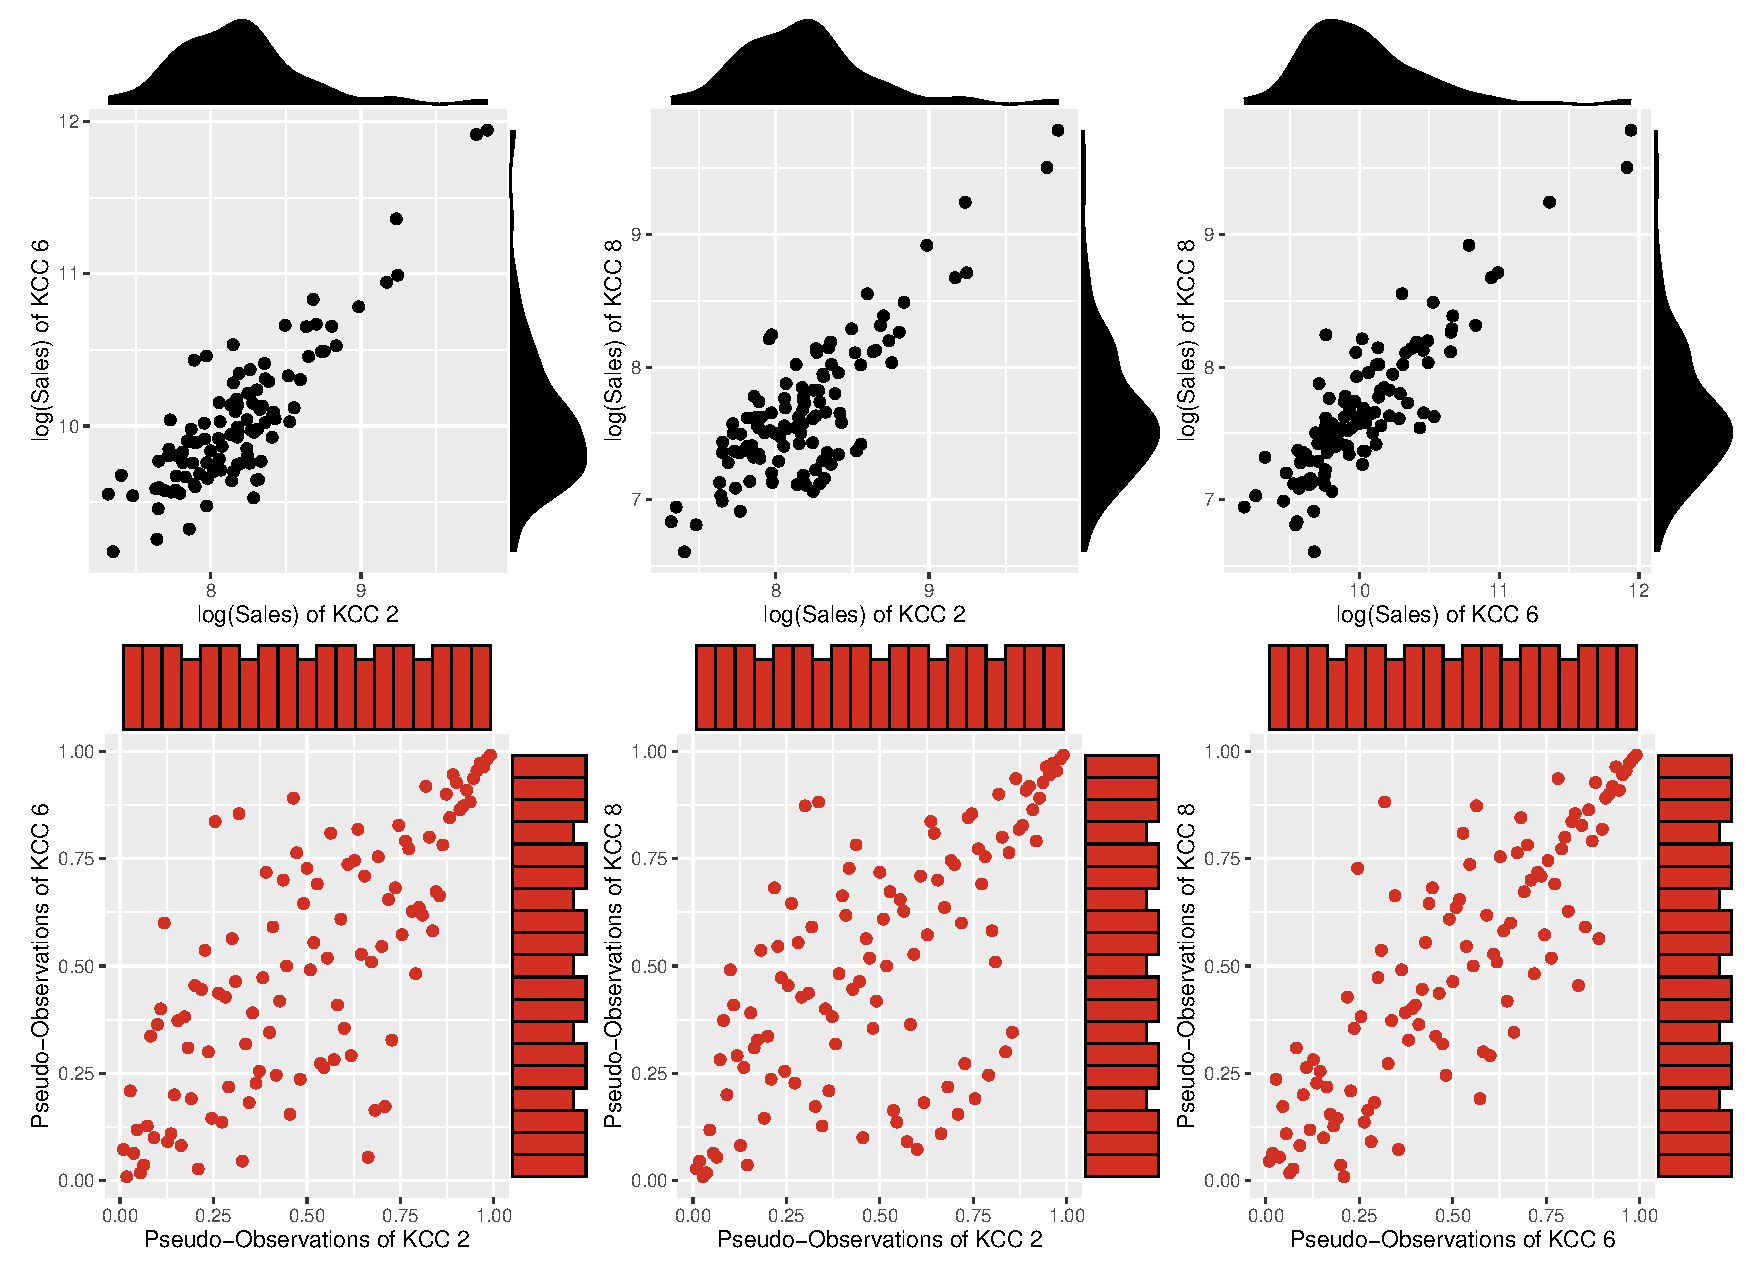
\includegraphics[width=0.95\linewidth]{figures/kcc_pair_scatterplots.eps}
  \caption{Pairwise scatterplots of sales on \ac{KCC} level. First row: Logarithmic sales with marginal densities, Second row: Pseudo sales observation with marginal histograms}
  \label{fig:kcc_pair_scatterplots}
\end{figure}


What is of more interest are the joint distributions of our \acp{KCC}. \autoref{fig:kcc_pair_scatterplots} shows scatterplots of \ac{KCC} pairs. In the first row we can see some isolated points on the upper tails representing outliers. We took the logarithmized sales to spot differences that would be otherwise hard to see. The outliers produced by the promotions still remain outliers in the log-scale. Also, by checking the densities for the marginals, pertinent marginal distributions are hardly determined but not to be ruled out.\\
The second row displays the pairs of the according \textit{pseudo observations}. Pseudo observations are calculated by taking the data ranks and dividing them by (1 + number of observations), which makes them robust against outliers and restricts the value range to $(0, 1)$. Here we are faced with a strange behaviour of the histograms. They look virtually uniformly distributed, however there are seemingly regular step patterns in the pseudo data. This might be traced back to the fact that we are dealing in reality with discrete data of not necessarily unique occurrence.\\

For the above reasons, on \ac{KCC} level we will attempt modelling parametric distributions to the marginals as well as directly use the pseudo data. The reason being for the latter is that our primary objective is to capture a dependence structure, whereas the marginals per se are of secondary interest. In addition, looking at both rows of \autoref{fig:kcc_pair_scatterplots}, we suspect tail dependence and there is an obvious strong positive correlation among all three pairs, which is confirmed by viewing \autoref{fig:corplot_kcc}. \\


\begin{figure}[H]
\centering
  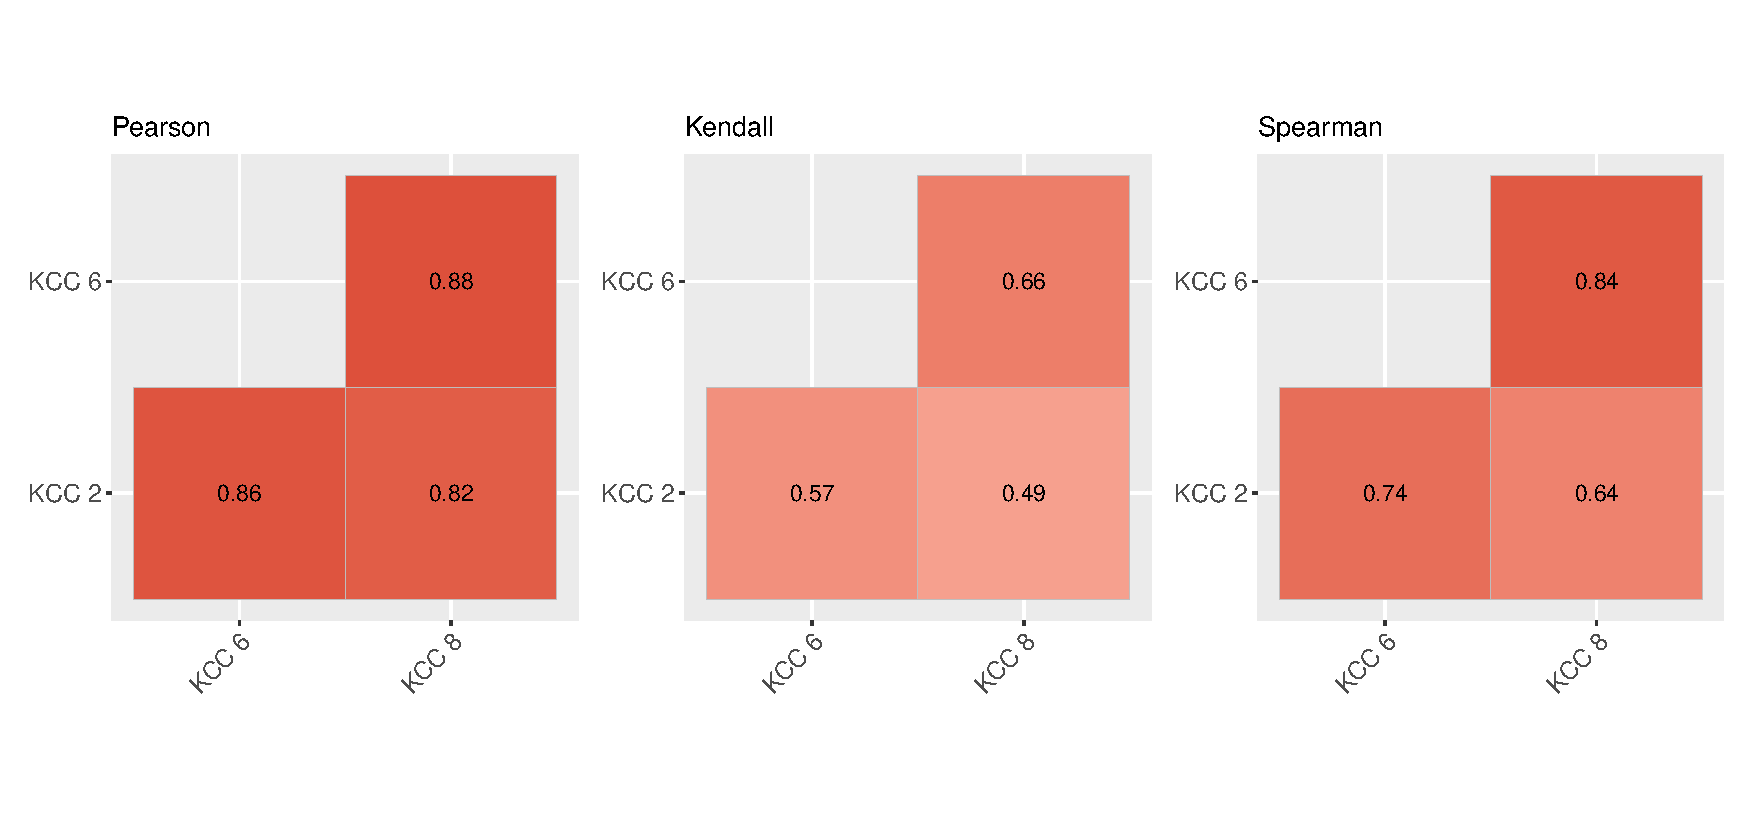
\includegraphics[width=0.95\linewidth]{figures/corplot_kcc.eps}
  \caption{Correlation plots of the three \ac{KCC} log-sales with different correlation coefficients. Left: Pearson's rho, Middle: Kendall's tau, Right: Spearman's rho}
  \label{fig:corplot_kcc}
\end{figure}

